\begin{frame}[fragile]{HTTP POST}
\begin{Verbatim}[fontsize=\small]
POST /cs4457-fall2024-quiz-listener.php HTTP/1.1
Host: kytos02-noauth.cs.virginia.edu
Content-Type: application/json
Content-Length: 184
...

{"user":"cr4bd","realuser":"cr4bd","session_id":"abcdefabcdef0123456789aaaaaaaaaaaaaaaaaaaaaaaaaaaaaaaaaaaaaaaaaa","quiz":"week09","slug":"71d45222","answer":["d2f4e81b"],"sequence":0}
\end{Verbatim}
\end{frame}

\begin{frame}[fragile]{HTML forms (GET)}
\begin{tikzpicture}
\node[align=left,font=\fontsize{8}{9}\selectfont] (html) {
\begin{minipage}{0.6\textwidth}
\begin{Verbatim}
<form action="https://example.com/foo" method="get">
Name: <input type="text" name="name"><br>
Query: <input type="text" name="query"><br>
<input type="submit" value="Submit">
</form>
\end{Verbatim}
\end{minipage}
};
\node[anchor=north east] (pic) at (html.north west) {
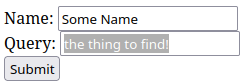
\includegraphics[width=0.3\textwidth]{../http/html-form-get.png}
};
\end{tikzpicture}
\begin{Verbatim}[fontsize=\small]
GET /foo?name=Some+Name&query=the+thing+to+find%21 HTTP/1.1
Host: example.com
...
\end{Verbatim}
\end{frame}

\begin{frame}[fragile]{HTML forms (POST)}
\begin{tikzpicture}
\node[align=left,font=\fontsize{8}{9}\selectfont] (html) {
\begin{minipage}{0.6\textwidth}
\begin{Verbatim}
<form action="https://example.com/foo" method="post">
Name: <input type="text" name="name"><br>
Comment:
<textarea name="comment">
</textarea>
<br>
<input type="submit" value="Submit">
</form>
\end{Verbatim}
\end{minipage}
};
\node[anchor=north east] (pic) at (html.north west) {
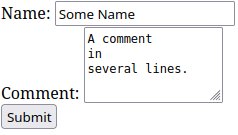
\includegraphics[width=0.3\textwidth]{../http/html-form-post.png}
};
\end{tikzpicture}
\begin{Verbatim}[fontsize=\small]
POST /foo HTTP/1.1
Host: example.com
Content-Type: application/x-www-form-urlencoded
Content-Length: 60
...

name=Some+Name&comment=A+comment%0D%0Ain%0D%0Aseveral+lines.
\end{Verbatim}
\end{frame}

\begin{frame}[fragile]{HTML forms (multipart/form-data)}
\begin{Verbatim}[fontsize=\fontsize{9}{10}]
<form action="https://example.com/foo" method="post"
    enctype="multipart/form-data">
    ...
\end{Verbatim}
\rule{0.9\textwidth}{1mm}
\begin{Verbatim}[fontsize=\fontsize{9}{10}]
POST /foo HTTP/1.1
Host: example.com
Content-Type: multipart/form-data; boundary=---------------------------81545828010202052201987031310
Content-Length: 321
...

-----------------------------30871118663472832060210928793
Content-Disposition: form-data; name="name"

Some Name
-----------------------------30871118663472832060210928793
Content-Disposition: form-data; name="comment"

A comment
in
several lines.
-----------------------------30871118663472832060210928793--
\end{Verbatim}
\end{frame}

\begin{frame}{GET v POST}
\begin{tabular}{p{7cm}|p{7cm}}
GET & POST \\ \hline
works with back button, caches & not resent automatically \\
limited by URL size & huge possible size \\
saving URL accesses page again & form info never `leaked' in browser history, referer, etc.\\
only simple text fields & supports file uploads (via multipart/form-data) \\
\end{tabular}
\end{frame}

